\documentclass{article}
\usepackage[margin=3.5cm]{geometry}   
\usepackage{tikz,amsmath}
\usetikzlibrary{arrows,shapes,positioning,shadows,trees}
\usepackage[
  colorlinks=true,
  urlcolor=cyan!70!black
  ]{hyperref}
	
\title{Homework II}
\author{Gregory Williams\\GW4975\\EE 382C Program Management}
\date{10/09/2015}

\begin{document}
	\maketitle
	\section*{Problem 9.14}
	
	\begin{center}
	\makebox[\textwidth]{
		
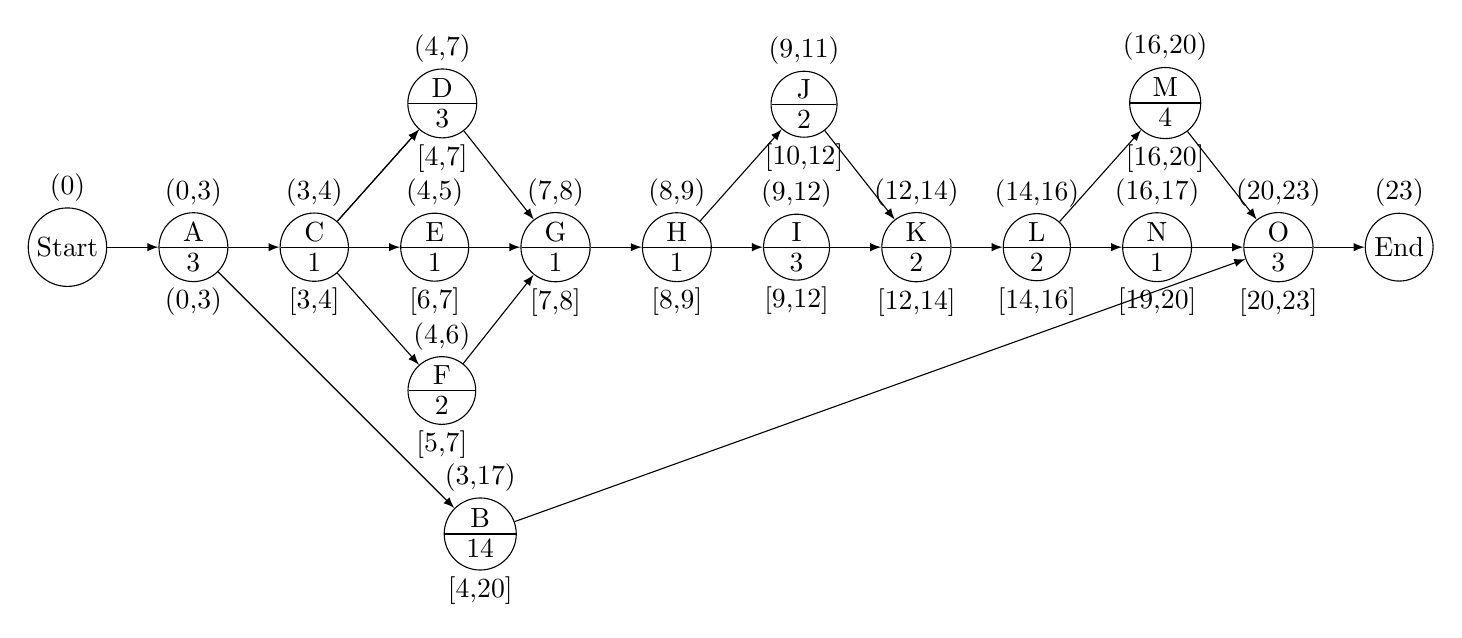
\begin{tikzpicture}[
  >=latex,
  every node/.style={draw,inner sep=2pt,minimum size=1pt},
  scale=0.5,
  node distance=.65cm,
  ]
  \node[circle, label=90:(0),] (S){Start};
  \node[circle split, right = of S, label=90:{(0,3)}, label=270:{(0,3)}] (A) {A \nodepart{lower} 3};
  \node[circle split, below right = 3 and 3 of A, label=90:{(3,17)}, label=270:{[4,20]}] (B) {B \nodepart{lower} 14};
  \node[circle split, right = of A, label=90:{(3,4)}, label=270:{[3,4]}] (C) {C \nodepart{lower} 1};
  \node[circle split, above right = 1.2 and 1 of C, label=90:{(4,7)}, label=270:{[4,7]}] (D) {D \nodepart{lower} 3};
  \node[circle split, right = of C, label=90:{(4,5)}, label=270:{[6,7]}] (E) {E \nodepart{lower} 1};
  \node[circle split, below right = 1.2 and 1 of C, label=90:{(4,6)}, label=270:{[5,7]}] (F) {F \nodepart{lower} 2};
  \node[circle split, right = of E, label=90:{(7,8)}, label=270:{[7,8]}] (G) {G \nodepart{lower} 1};
  \node[circle split, right = of G, label=90:{(8,9)}, label=270:{[8,9]}] (H) {H \nodepart{lower} 1};
  \node[circle split, right = of H, label=90:{(9,12)}, label=270:{[9,12]}] (I) {I \nodepart{lower} 3};
  \node[circle split, above right = 1.2 and 1 of H, label=90:{(9,11)}, label=270:{[10,12]}] (J) {J \nodepart{lower} 2};
  \node[circle split, right = of I, label=90:{(12,14)}, label=270:{[12,14]}] (K) {K \nodepart{lower} 2};
  \node[circle split, right = of K, label=90:{(14,16)}, label=270:{[14,16]}] (L) {L \nodepart{lower} 2};
  \node[circle split, above right = 1.2 and 1 of L, label=90:{(16,20)}, label=270:{[16,20]}] (M) {M \nodepart{lower} 4};
  \node[circle split, right = of L, label=90:{(16,17)}, label=270:{[19,20]}] (N) {N \nodepart{lower} 1};
  \node[circle split, right = of N, label=90:{(20,23)}, label=270:{[20,23]}] (O) {O \nodepart{lower} 3};
  \node[circle, right = of O, label=90:{(23)}] (End) {End};
  
  
  \draw [->] (S) -- (A);
  \draw [->] (A) -- (B);
  \draw [->] (A) -- (C);
  \draw [->] (C) -- (D);
  \draw [->] (C) -- (E);
  \draw [->] (C) -- (F);
  \draw [->] (D) -- (G);
  \draw [->] (E) -- (G);
  \draw [->] (F) -- (G);
  \draw [->] (G) -- (H);
  \draw [->] (H) -- (I);
  \draw [->] (H) -- (J);
  \draw [->] (C) -- (D);
  \draw [->] (I) -- (K);
  \draw [->] (J) -- (K);
  \draw [->] (K) -- (L);
  \draw [->] (L) -- (M);
  \draw [->] (L) -- (N);
  \draw [->] (B) -- (O);
  \draw [->] (M) -- (O);
  \draw [->] (N) -- (O);
  \draw [->] (O) -- (End);
  
\end{tikzpicture}

}
	\end{center}
	Critical path: A-C-D-G-H-I-K-L-M-O \\
	Duration: 23 days
	\pagebreak
	\section*{Problem 9.15}
	
	{\renewcommand{\arraystretch}{1.2} 
	\begin{table}[h!tbp]
  		\begin{center}
    		\caption{Slacks for Buying Tom Cruise a Boat}
    		\label{tab:table1}
			
    		\begin{tabular}{lcccc}
				Activity & Total Slack Eq & Total Slack & Free Slack Eq & Total Slack\\
				& LS - ES & & Min\{ES$_{\text{Suc}}$\} - EF & \\
				\hline
      			A* & & 0 & & 0\\
      			B & 20-17= & 3 & 20-17= & 3\\
				C* && 0 && 0\\
				D* && 0 && 0\\
				E & 7-5= & 2 & 7-5= & 2\\
				F & 7-6= & 1 & 7-6= & 1\\
				G* && 0 && 0\\
				H* && 0 && 0\\
				I* && 0 && 0\\
				J & 12-11= & 1 & 12-11= & 1\\
				K* && 0 && 0\\
				L* && 0 && 0\\
				M* && 0 && 0\\
				N & 20-17= & 3 & 20-17= & 3\\
				O* && 0 && 0\\
				\hline
				\multicolumn{3}{c}{* = On the Critical Path}\\
    		\end{tabular}
  		\end{center}
	\end{table}
	}
	
	\section*{Problem 9.19}
	
	\section*{Problem 9.20}
		
	\section*{Problem 9.22}
	
	\section*{Problem 9.23}
	
\end{document}